\section{Introduction}

This document describes the calibration procedure for White Rabbit devices. 

A White Rabbit link established between two devices is characterized by the
hardware delays and fiber propagation latencies presented in figure
\ref{fig:intro:link-model}.

\begin{figure}[ht]
	\begin{center}
		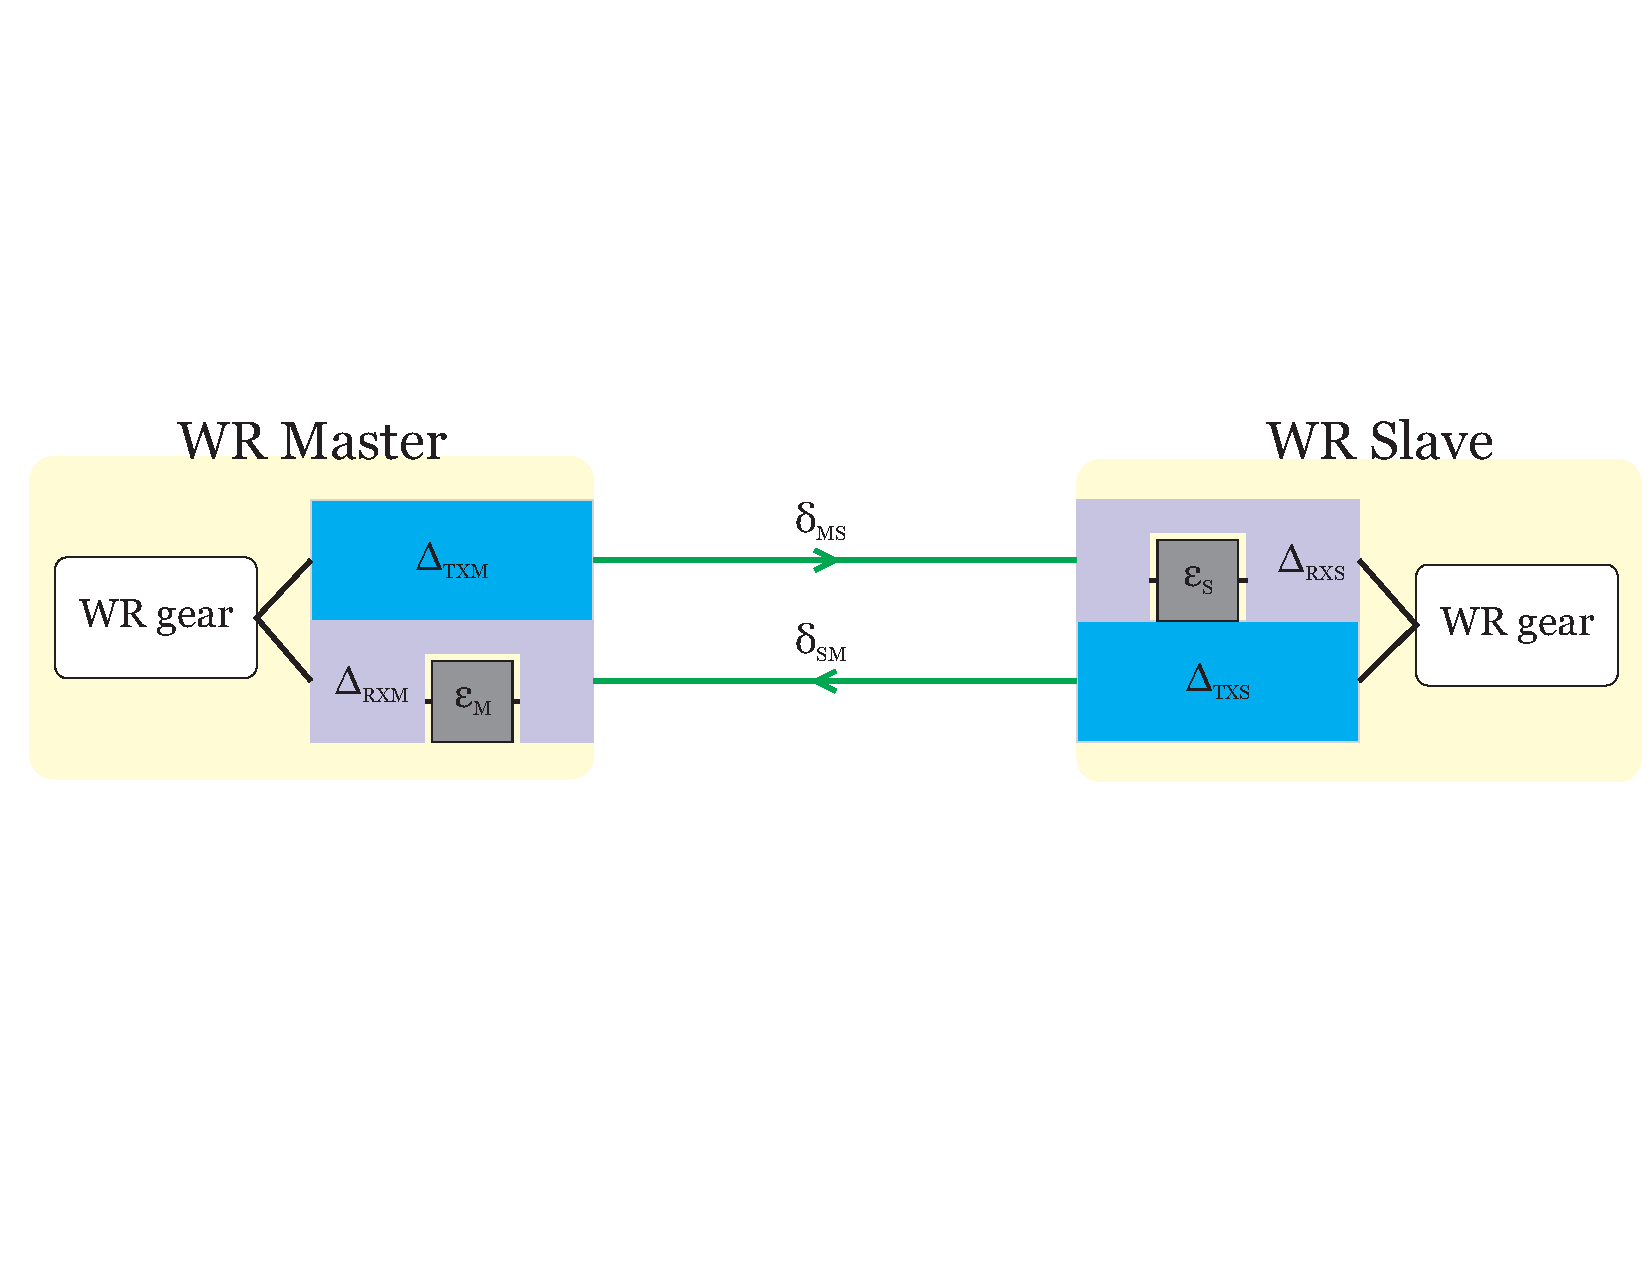
\includegraphics[width=\textwidth]{calibration/link-model.pdf}
		\caption{White Rabbit link model}
		\label{fig:intro:link-model}
	\end{center}
\end{figure}

Each WR Master and WR Slave has some constant transmission and reception delays
($\Delta_{TXM}$, $\Delta_{RXM}$, $\Delta_{TXS}$, $\Delta_{RXS}$). They are the
summed result of SFP transceiver, PCB trace and electronic component
delays as well as the delays inside the FPGA chip. Additional reception delay is
also caused on both sides by aligning the recovered clock signal to the inter-symbol
boundaries of the data stream. This is called the bitslide value and is marked in figure
\ref{fig:intro:link-model} as $\epsilon_M$ and $\epsilon_S$.

In addition to hardware delays, packets transmitted in fiber are affected with
propagation latencies in both directions ($\delta_{MS}$, $\delta_{SM}$). These
fiber propagation latencies are not equal since different light wavelengths are 
used to communicate simultaneously in both directions using a single fiber.

Based on those parameters the round-trip delay ($delay_{MM}$) is defined as the
sum of all delay factors described above:
\begin{equation}
	delay_{MM} = \Delta_{TXM} + \Delta_{RXS} + \epsilon_S + \Delta_{TXS} +
	\Delta_{RXM} + \epsilon_M + \delta_{MS} + \delta_{SM}
\end{equation}

However, since the bitslide values can be easily obtained from WR software, 
the calibration procedure described in this document use a modified round-trip delay, 
without $\epsilon_M$ and $\epsilon_S$:
\begin{equation}
	delay_{MM}' = delay_{MM} - \epsilon_M - \epsilon_S
\end{equation}

In the synchronization process, the PTP daemon tries to calculate the current
offset between Slave and Master clock. For that it needs a precise estimation of
the one-way link delay which, using the described link model, is the sum of four
factors:
\begin{equation}
	delay_{MS} = \Delta_{TXM} + \delta_{MS} + \Delta_{RXS} + \epsilon_S
\end{equation}

The calibration procedure described in this document is required since the
values of the hardware transmission and reception delays are not known
($\Delta_{TXM}$, $\Delta_{RXM}$, $\Delta_{TXS}$, $\Delta_{RXS}$). Moreover, 
fiber cable and each device has unknown asymmetry that prevents from estimating 
$delay_{MS}$ as half of the round-trip $delay_{MM}$.
